\section{实验结果与分析}

\subsection{生成数据}

为了保证生成的数据满足朴素贝叶斯假设,$raw\_data()$函数保证相同类别的向量$\mathbf{X}^l$,其各个维度都有
\begin{eqnarray}
    x^l_i \sim \mathcal{N} \left(\mu, \sigma\right)
\end{eqnarray}
即各个维度$x^l_i$都服从各自的正态分布。

生成的两类数据如图\ref{gen_data}。

\begin{figure}[htbp]
    \centering
    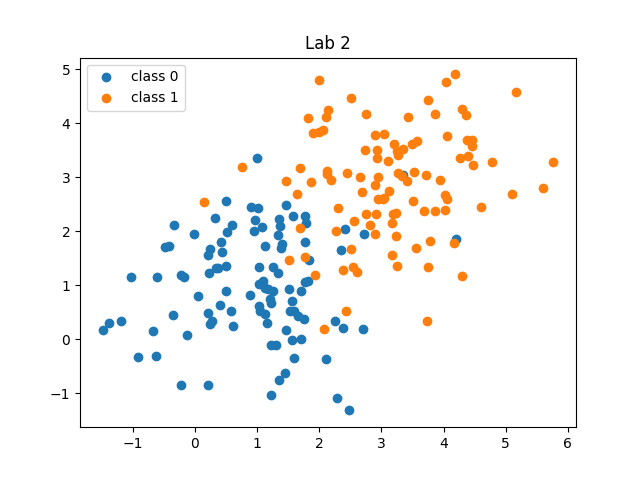
\includegraphics[width=0.7\textwidth]{figures/Figure_1.png}
    \caption{生成两类数据}
    \label{gen_data}
\end{figure}

\subsection{梯度下降法确定分类面}

使用梯度下降法迭代$10000$次,确定分类面系数$\mathbf{w}$,从而获得了分类面方程
\begin{equation}
    \label{sep_equ}
    \mathbf{w}^T\mathbf{X}=0
\end{equation}

对于一个二维向量的原始数据,方程\ref{sep_equ}也可写为
\begin{equation}
    w_0 + w_1 x + w_2 y = 0
\end{equation}
由此可以作出二维平面上的分类面图像,如图\ref{sep_equ_figure}。

\begin{figure}[htbp]
    \centering
    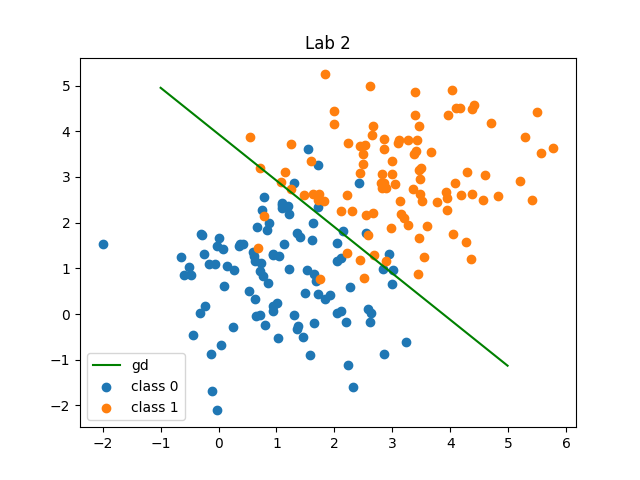
\includegraphics[width=0.7\textwidth]{figures/Figure_2.png}
    \caption{分类面}
    \label{sep_equ_figure}
\end{figure}

绘制出分类面后,同样可以计算分类误差。计算方式为
\begin{equation}
    loss = \dfrac{count_{01}}{count_0}
\end{equation}
即:类别$0$的点,分到类别$1$的个数$/$类别$0$的点的总个数

图\ref{sep_equ_figure}所示的分类面,其分类所需的迭代次数及误差如图\ref{loss}

\begin{figure}[htbp]
    \centering
    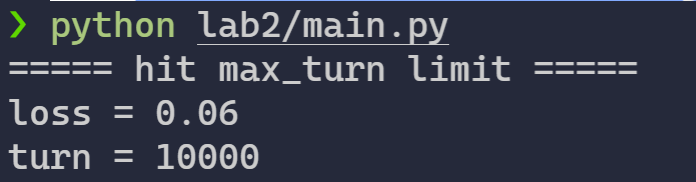
\includegraphics[width=0.7\textwidth]{figures/Figure_3.png}
    \caption{分类面误差}
    \label{loss}
\end{figure}

\subsection{加入正则项}

对于逻辑回归的
\begin{equation}
    \mathbf{w}^T\mathbf{X}=0
\end{equation}
的分类面的形式,对于实验中的2维向量并不会出现过拟合现象。因此在此处加入正则项只是简化了模型的复杂度。

采取与实验一类似的方式,从一个较小的值开始依次计算正则项系数$\lambda$可能取到的值,比较各自的loss,从而选取一个最合适的$\lambda$。

图\ref{lambda20}和图\ref{lambda100}分别展示了样本数据量为$40$和$100$时、$\lambda$为$0.01$时的分类效果(如图中红色直线所示)。绿色直线为不加入正则项,而红色直线为加入正则项,图中可见二者几乎重叠,因此在此处是否加入正则项对分类的精度几乎无影响。

\begin{figure}[htbp]
    \begin{minipage}[t]{0.5\linewidth}
        \centering
        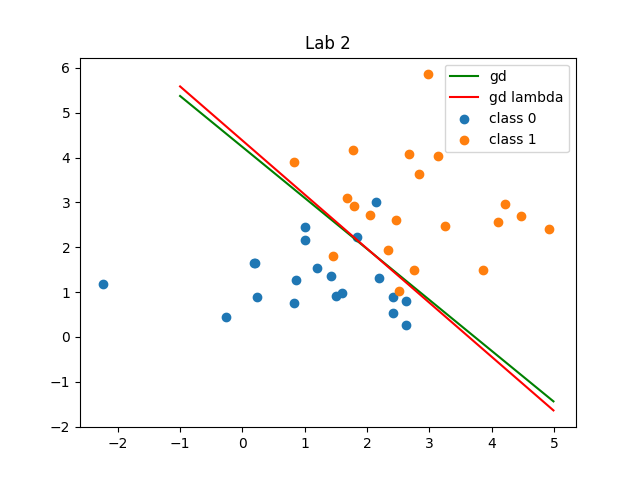
\includegraphics[width=\textwidth]{figures/Figure_4.png}
        \caption{每个类别的样本数量为$20$时的情况}
        \label{lambda20}
    \end{minipage}
    \begin{minipage}[t]{0.5\linewidth}
        \centering
        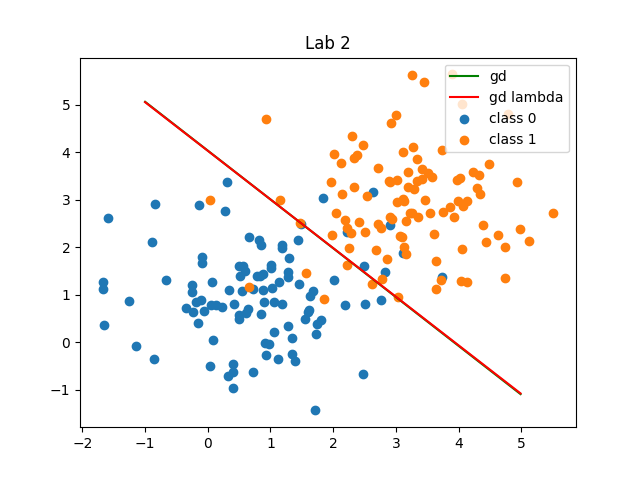
\includegraphics[width=\textwidth]{figures/Figure_5.png}
        \caption{每个类别的样本数量为$100$时的情况}
        \label{lambda100}
    \end{minipage}
\end{figure}

\subsection{破坏朴素贝叶斯假设}

破坏生成的数据中的朴素贝叶斯假设。$raw\_data\_dim2()$保证向量的第一个维度(即$x$)服从正态分布,而第二个维度(即$y$)是一个值与$x$的差,这样$x$和$y$的相关系数就是$-1$。绘制原始数据和分类面,如图\ref{no-native}。

\begin{figure}[htbp]
    \begin{minipage}[t]{0.5\linewidth}
        \centering
        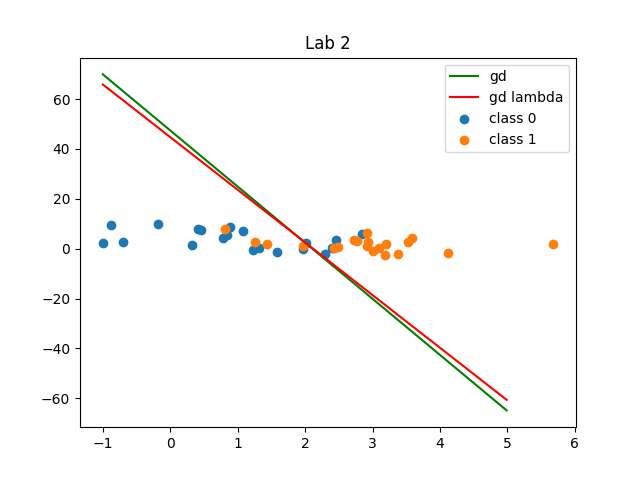
\includegraphics[width=\textwidth]{figures/Figure_6.png}
        \caption{不满足朴素贝叶斯假设的原始数据,使用逻辑回归进行分类}
        \label{no-native}
    \end{minipage}
    \begin{minipage}[t]{0.5\linewidth}
        \centering
        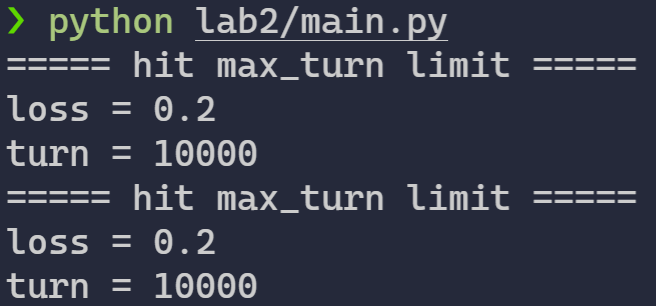
\includegraphics[width=\textwidth]{figures/Figure_7.png}
        \caption{不满足朴素贝叶斯假设的分类误差。其中第一个loss是不含正则项的误差,第二个loss是带有正则项的误差}
        \label{no-native-loss}
    \end{minipage}
\end{figure}

分类后的误差如图\ref{no-native-loss},与图\ref{loss}相比,分类效果并不好。

\subsection{UCI网站数据分类}

使用的数据为钞票数据集Banknote Dataset\cite{uci}。这是从纸币鉴别过程中的图像里提取的数据,用来预测钞票的真伪的数据集。样本中的每一行有5个数值,分别是4个输入和1个输出,其意义分别为:

第一列:图像经小波变换后的方差

第二列:图像经小波变换后的偏态

第三列:图像经小波变换后的峰度

第四列:图像的熵

第五列:钞票所属的类别(0或1)。

因此,在逻辑回归中,上述样本的前四项可以看作是一个4维向量,而最后一列则是这个向量的类别。使用逻辑回归对给定的样本进行分类,由于4维向量不便于展示,此处仅给出分类的误差分析,如图\ref{uci}。

\begin{figure}[htbp]
    \centering
    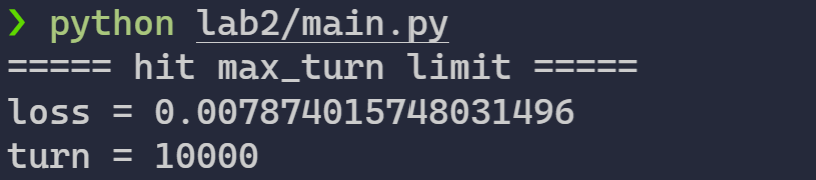
\includegraphics[width=0.7\textwidth]{figures/Figure_8.png}
    \caption{使用逻辑回归对UCI钞票数据集进行分类的误差}
    \label{uci}
\end{figure}

可见分类效果良好。
